\documentclass[a4paper,12pt,openany,oneside]{book} % kodovanie diakritiky je utf-8
\usepackage[utf8]{inputenc}
\usepackage[slovak]{babel}
\usepackage{a4wide,color}
\usepackage[top=2.5cm, bottom=2.5cm, left=2.75cm, right=2.75cm]{geometry}
%\usepackage[top=2.5cm, bottom=2.5cm, left=3.5cm, right=2cm]{geometry}
\usepackage{lmodern}
\usepackage[T1]{fontenc}
\usepackage{fontenc}
\usepackage{amsfonts}
\usepackage{amssymb}
\usepackage{amsthm}
\usepackage{epsfig}
\usepackage{wrapfig}
\usepackage{graphicx}
\usepackage{caption}
\usepackage{subcaption}
\usepackage{url}
\usepackage[bookmarks]{hyperref}

\usepackage{pdfpages}
\usepackage{listings}
\renewcommand\baselinestretch{1.3} % riadkovanie jeden a pol

\definecolor{dkgreen}{rgb}{0,0.6,0}
\definecolor{gray}{rgb}{0.5,0.5,0.5}
\definecolor{mauve}{rgb}{0.58,0,0.82}
 
\lstset{ %
  language=C++,                % the language of the code
  basicstyle=\footnotesize,           % the size of the fonts that are used for the code
  numbers=left,                   % where to put the line-numbers
  numberstyle=\tiny\color{gray},  % the style that is used for the line-numbers
  stepnumber=1,                   % the step between two line-numbers. If it's 1, each line 
                                  % will be numbered
  numbersep=5pt,                  % how far the line-numbers are from the code
  backgroundcolor=\color{white},      % choose the background color. You must add \usepackage{color}
  showspaces=false,               % show spaces adding particular underscores
  showstringspaces=false,         % underline spaces within strings
  showtabs=false,                 % show tabs within strings adding particular underscores
  frame=single,                   % adds a frame around the code
  rulecolor=\color{black},        % if not set, the frame-color may be changed on line-breaks within not-black text (e.g. commens (green here))
  tabsize=2,                      % sets default tabsize to 2 spaces
  captionpos=b,                   % sets the caption-position to bottom
  breaklines=true,                % sets automatic line breaking
  breakatwhitespace=false,        % sets if automatic breaks should only happen at whitespace
  title=\lstname,                   % show the filename of files included with \lstinputlisting;
                                  % also try caption instead of title
  keywordstyle=\color{blue},          % keyword style
  commentstyle=\color{dkgreen},       % comment style
  stringstyle=\color{mauve},         % string literal style
  escapeinside={\%*}{*)},            % if you want to add a comment within your code
  morekeywords={*,...}               % if you want to add more keywords to the set
}

% pekne pokope definujeme potrebne udaje
\def\mftitle{Konštrukcia grafov pomocou mobilných agentov}
\def\mftitlefirst{Konštrukcia grafov pomocou mobilných agentov}
\def\mftitlesecond{}
\def\mfthesistype{Diplomová práca}
\def\mfauthor{Bc. Jakub Kováč}
\def\mfadvisor{prof. RNDr. Rastislav Kráľovič, PhD.}
\def\mfdate{2014}
\def\mfplacedate{Bratislava, \mfdate}
\def\mfuniversity{Univerzita Komenského, Bratislava}
\def\mffakulta{Fakulta Matematiky, Fyziky a Informatiky}
% \ifx\pdfoutput\undefined\relax\else\pdfinfo{ /Title (\mftitle) /Author (\mfauthor) /Creator (PDFLaTeX) } \fi

\def\todo{{\color{red} TODO!!!}}
\def\method#1{{\tt #1}}

\ifpdf
  \pdfinfo{
    /Title (\mftitle)
    /Author (\mfauthor)
    /Creator (PDFLaTeX)
  }
\else
\fi

\begin{document}

\frontmatter

\thispagestyle{empty}

\noindent
%\begin{minipage}{0.20\textwidth}
%
\includegraphics[width=0.9\textwidth]{komlogo-new}
%\end{minipage}
\begin{center}
\begin{minipage}{0.8\textwidth}
\centerline{\renewcommand\baselinestretch{1.3} \LARGE\sc\mfuniversity}
\centerline{\sc\mffakulta}
\end{minipage}
\end{center}

\vfill
\begin{center}
\begin{minipage}{1\textwidth}
%\hrule
\bigskip\bigskip
\begin{center}
\linespread{1}\LARGE\sc\mftitle
\end{center}
\smallskip
\centerline{\mfthesistype}
\bigskip
\bigskip
%\centerline{\large\sc\mfauthor}
\bigskip\bigskip
%\hrule
\end{minipage}
\end{center}
\vfill
{\bf\mfdate\\
\indent\mfauthor}
%{\bf Vedúci:} \mfadvisor
\eject % EOP i

% \thispagestyle{empty}~\vfill\eject % EOP ii % zadna strana obalu je prazdna

\thispagestyle{empty}

\noindent
%\begin{minipage}{0.20\textwidth}
%
\includegraphics[width=0.9\textwidth]{komlogo-new}
%\end{minipage}
\begin{center}
\begin{minipage}{0.8\textwidth}
\centerline{\LARGE\sc\mfuniversity}
\centerline{\sc\mffakulta}
\end{minipage}
\end{center}

\vfill
\begin{center}
\begin{minipage}{1\textwidth}
%\hrule
\bigskip\bigskip
\begin{center}
\linespread{1}\LARGE\sc\mftitle
\end{center}
\smallskip
\centerline{\mfthesistype}
\bigskip
\bigskip
%\centerline{\large\sc\mfauthor}
\bigskip\bigskip
%\hrule
\end{minipage}
\end{center}
\vfill
\begin{minipage}{0.8\textwidth}
\begin{tabular}{l l}
Študijný program:& Informatika \\
Študijný odbor:& 2508 Informatika \\
Školiace pracovisko:& Katedra Informatiky\\
Školiteľ:&   \mfadvisor \\
\end{tabular}
\end{minipage}
\begin{center}
\end{center}
\vfill
{\bf\mfplacedate\\
\indent\mfauthor}
%{\bf Vedúci:} \mfadvisor
\eject % EOP iii

% \thispagestyle{empty}~\vfill\eject % EOP iv % zadna strana titulky je prazdna

% {~}\vspace{12cm}
% 
% \noindent
% \begin{minipage}{0.25\textwidth}~\end{minipage}
% \begin{minipage}{0.68\textwidth}
% Čestne prehlasujem, že som túto diplomovú prácu vypracoval(a) samostatne s použitím citovaných zdrojov.
% 
% \bigskip\bigskip
% 
% \hfill\hbox to 6cm{\dotfill}
% \end{minipage}
% \vfill\eject % EOP v
% ~\vfill\eject % EOP vi % zadna strana prehlasenia je prazdna

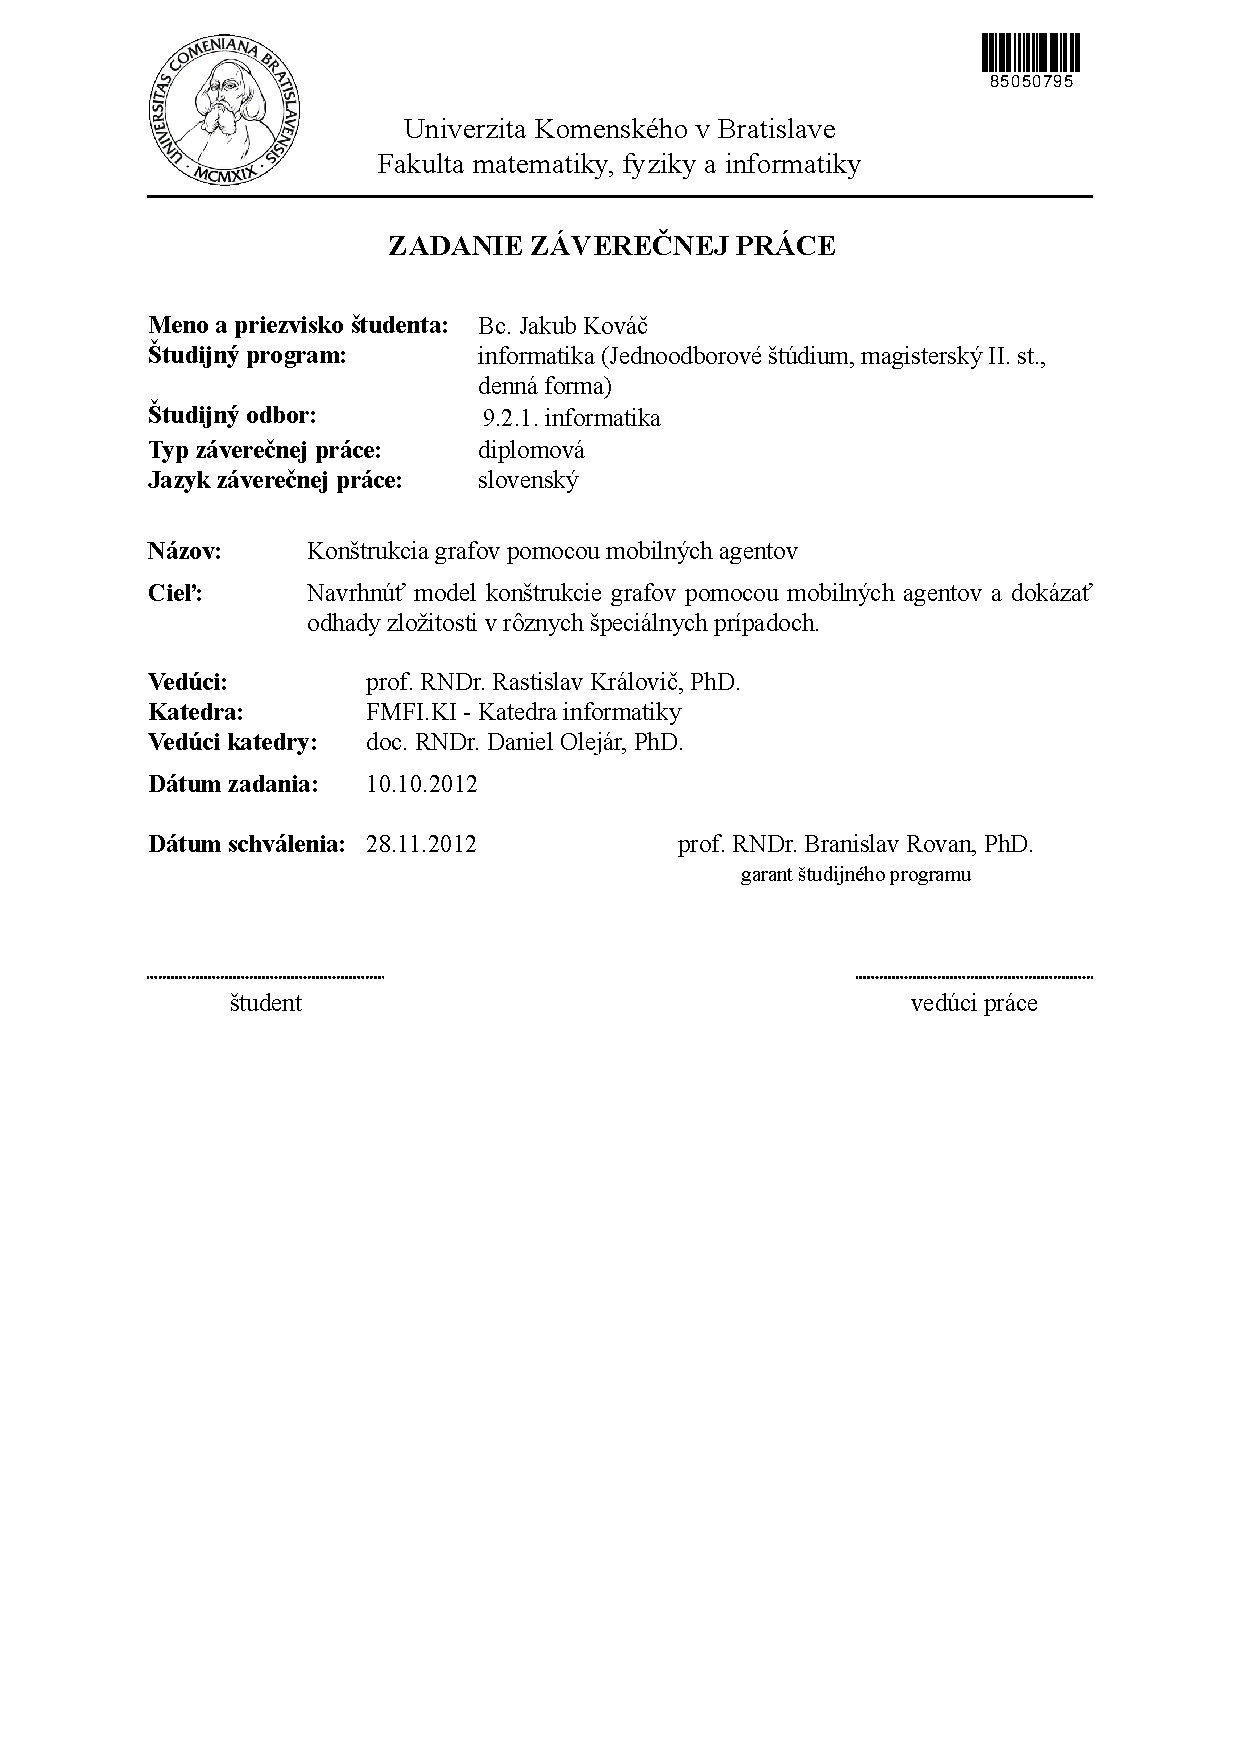
\includepdf{zadanie.pdf}

{~}\vspace{12cm}

%\noindent
%\begin{minipage}{0.25\textwidth}~\end{minipage}
%\begin{center}
%\begin{minipage}{1\textwidth}
%Ďakujem vedúcemu bakalárskej práce Marekovi Nagyovi za cenné rady 
%a pripomienky, bez ktorých by táto práca asi nevznikla, priateľke, blízkym priateľom a rodine za morálnu podporu.
%\end{minipage}
%\end{center}
%\hfill\mfauthor
%\vfill\eject % EOP v

% ~\vfill\eject % EOP vi % zadna strana prehlasenia je prazdna


\noindent
%\begin{minipage}{0.25\textwidth}~\end{minipage}
\begin{center}
\begin{minipage}{1\textwidth}
\centerline{\large Abstrakt}
%\begin{center}
\input abstrakt.tex
\\ \\ 
{\bf Kľúčové slová:} konštrukcia grafov, agent, anonymný garf, hyperkocka, 
 prehľadávanie grafov, grafové gramatiky
%\end{center}
\end{minipage}
\end{center}
\eject % EOP v
% ~\vfill\eject % EOP vi % zadna strana prehlasenia je prazdna

\noindent
%\begin{minipage}{0.25\textwidth}~\end{minipage}
\begin{center}
\begin{minipage}{1\textwidth}
\centerline{\large Abstract}
%\begin{center}
\input abstractEN.tex
\\ \\
{\bf Key words:} graph constructions, agent, robot, anonymous graph,
hypercube, graph exploration, graph grammars
%\end{center}
\end{minipage}
\end{center}
\eject % EOP v
% ~\vfill\eject % EOP vi % zadna strana prehlasenia je prazdna

\noindent
\input predhovor.tex


\tableofcontents
\listoffigures
\listoftables

\mainmatter
\newtheorem{lem}{Lema}
\newtheorem{defin}{Definícia}
\newtheorem{veta}{Veta}
\newtheorem{pozn}{Poznámka}
\newtheorem{ozn}{Označenie}

%\input zac1.tex
%
\input uvod.tex
\input definicie.tex
\input teoruvod.tex
\input prehladavanie.tex
\input zac1.tex
\input mriezka.tex
\input lemy1.tex
\input zaver.tex
%\input platforma_jazyk_kniznice.tex
%\input neuralnet.tex
%\input navrh.tex
%\input experimenty.tex
%\input implementacia.tex
%\input zaver.tex

%\iffalse
\backmatter

%\cleardoublepage
\phantomsection
\addcontentsline{toc}{chapter}{Literatúra}
\nocite{*}
\bibliographystyle{alpha}
\bibliography{literatura.bib}
%\fi
\end{document}
